\documentclass[14pt]{extbook}
\usepackage{multicol, enumerate, enumitem, hyperref, color, soul, setspace, parskip, fancyhdr} %General Packages
\usepackage{amssymb, amsthm, amsmath, latexsym, units, mathtools} %Math Packages
\everymath{\displaystyle} %All math in Display Style
% Packages with additional options
\usepackage[headsep=0.5cm,headheight=12pt, left=1 in,right= 1 in,top= 1 in,bottom= 1 in]{geometry}
\usepackage[usenames,dvipsnames]{xcolor}
\usepackage{dashrule}  % Package to use the command below to create lines between items
\newcommand{\litem}[1]{\item#1\hspace*{-1cm}\rule{\textwidth}{0.4pt}}
\pagestyle{fancy}
\lhead{Makeup Progress Quiz 3}
\chead{}
\rhead{Version ALL}
\lfoot{1648-1753}
\cfoot{}
\rfoot{Summer C 2021}
\begin{document}

\begin{enumerate}
\litem{
Construct the lowest-degree polynomial given the zeros below. Then, choose the intervals that contain the coefficients of the polynomial in the form $x^3+bx^2+cx+d$.\[ 3 - 2 i \text{ and } -3 \]\begin{enumerate}[label=\Alph*.]
\item \( b \in [1.1, 4], c \in [-5.1, -3.6], \text{ and } d \in [-40, -32] \)
\item \( b \in [-0.4, 2], c \in [-2.9, 0.1], \text{ and } d \in [-9, -4] \)
\item \( b \in [-0.4, 2], c \in [3.2, 8.7], \text{ and } d \in [4, 7] \)
\item \( b \in [-6.7, -1], c \in [-5.1, -3.6], \text{ and } d \in [36, 41] \)
\item \( \text{None of the above.} \)

\end{enumerate} }
\litem{
Describe the end behavior of the polynomial below.\[ f(x) = 2(x - 9)^{3}(x + 9)^{8}(x - 7)^{3}(x + 7)^{5} \]\begin{enumerate}[label=\Alph*.]
\begin{multicols}{2}\item 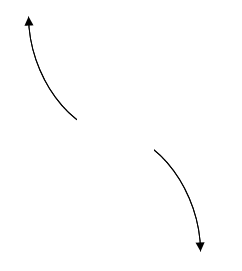
\includegraphics[width = 0.3\textwidth]{../Figures/polyEndBehaviorAA.png}\item 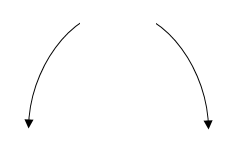
\includegraphics[width = 0.3\textwidth]{../Figures/polyEndBehaviorBA.png}\item 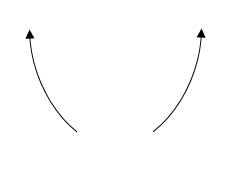
\includegraphics[width = 0.3\textwidth]{../Figures/polyEndBehaviorCA.png}\item 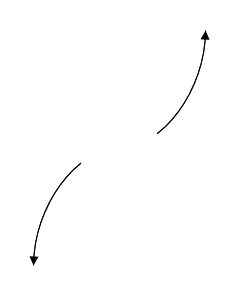
\includegraphics[width = 0.3\textwidth]{../Figures/polyEndBehaviorDA.png}\end{multicols}\item None of the above.
\end{enumerate} }
\litem{
Describe the end behavior of the polynomial below.\[ f(x) = -4(x - 2)^{5}(x + 2)^{10}(x - 3)^{5}(x + 3)^{6} \]\begin{enumerate}[label=\Alph*.]
\begin{multicols}{2}\item 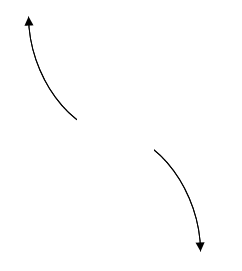
\includegraphics[width = 0.3\textwidth]{../Figures/polyEndBehaviorCopyAA.png}\item 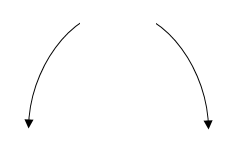
\includegraphics[width = 0.3\textwidth]{../Figures/polyEndBehaviorCopyBA.png}\item 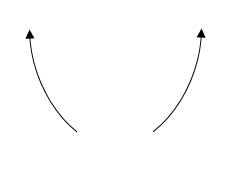
\includegraphics[width = 0.3\textwidth]{../Figures/polyEndBehaviorCopyCA.png}\item 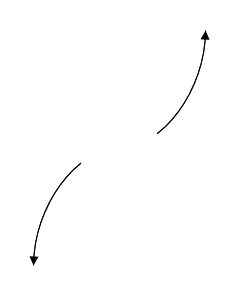
\includegraphics[width = 0.3\textwidth]{../Figures/polyEndBehaviorCopyDA.png}\end{multicols}\item None of the above.
\end{enumerate} }
\litem{
Construct the lowest-degree polynomial given the zeros below. Then, choose the intervals that contain the coefficients of the polynomial in the form $ax^3+bx^2+cx+d$.\[ -6, \frac{-3}{4}, \text{ and } \frac{7}{2} \]\begin{enumerate}[label=\Alph*.]
\item \( a \in [3, 10], b \in [-75, -66], c \in [108, 118], \text{ and } d \in [125, 128] \)
\item \( a \in [3, 10], b \in [-26, -24], c \in [-154, -145], \text{ and } d \in [125, 128] \)
\item \( a \in [3, 10], b \in [23, 33], c \in [-154, -145], \text{ and } d \in [-130, -119] \)
\item \( a \in [3, 10], b \in [-89, -77], c \in [222, 233], \text{ and } d \in [-130, -119] \)
\item \( a \in [3, 10], b \in [23, 33], c \in [-154, -145], \text{ and } d \in [125, 128] \)

\end{enumerate} }
\litem{
Describe the zero behavior of the zero $x = 3$ of the polynomial below.\[ f(x) = 6(x - 3)^{4}(x + 3)^{9}(x + 7)^{4}(x - 7)^{8} \]\begin{enumerate}[label=\Alph*.]
\begin{multicols}{2}\item 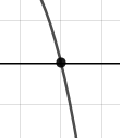
\includegraphics[width = 0.3\textwidth]{../Figures/polyZeroBehaviorAA.png}\item 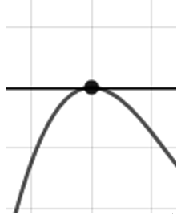
\includegraphics[width = 0.3\textwidth]{../Figures/polyZeroBehaviorBA.png}\item 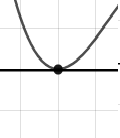
\includegraphics[width = 0.3\textwidth]{../Figures/polyZeroBehaviorCA.png}\item 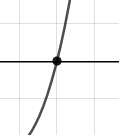
\includegraphics[width = 0.3\textwidth]{../Figures/polyZeroBehaviorDA.png}\end{multicols}\item None of the above.
\end{enumerate} }
\litem{
Which of the following equations \textit{could} be of the graph presented below?
\begin{center}
    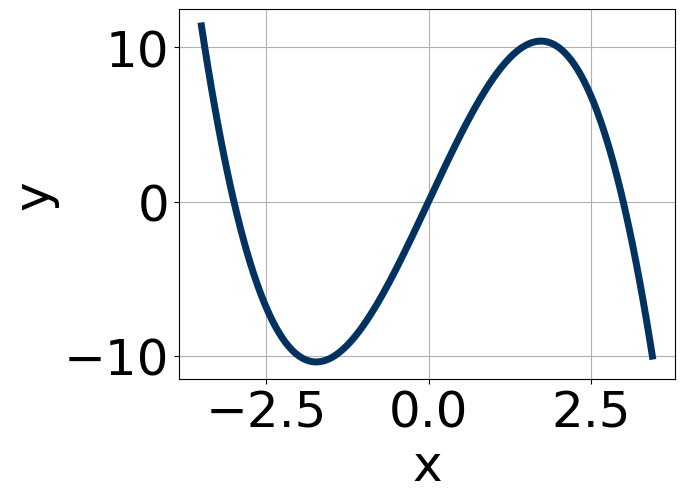
\includegraphics[width=0.5\textwidth]{../Figures/polyGraphToFunctionA.png}
\end{center}
\begin{enumerate}[label=\Alph*.]
\item \( 5x^{5} (x - 3)^{10} (x + 3)^{5} \)
\item \( -7x^{9} (x - 3)^{4} (x + 3)^{9} \)
\item \( -14x^{11} (x - 3)^{5} (x + 3)^{9} \)
\item \( -18x^{9} (x - 3)^{4} (x + 3)^{8} \)
\item \( 17x^{7} (x - 3)^{5} (x + 3)^{5} \)

\end{enumerate} }
\litem{
Construct the lowest-degree polynomial given the zeros below. Then, choose the intervals that contain the coefficients of the polynomial in the form $x^3+bx^2+cx+d$.\[ -2 - 5 i \text{ and } 3 \]\begin{enumerate}[label=\Alph*.]
\item \( b \in [0.2, 3.8], c \in [16.8, 19.7], \text{ and } d \in [-92, -81] \)
\item \( b \in [0.2, 3.8], c \in [-3.5, 0.3], \text{ and } d \in [-9, -3] \)
\item \( b \in [-4.5, 0.5], c \in [16.8, 19.7], \text{ and } d \in [86, 92] \)
\item \( b \in [0.2, 3.8], c \in [1.8, 4.3], \text{ and } d \in [-18, -11] \)
\item \( \text{None of the above.} \)

\end{enumerate} }
\litem{
Describe the zero behavior of the zero $x = 5$ of the polynomial below.\[ f(x) = -9(x - 6)^{11}(x + 6)^{9}(x - 5)^{7}(x + 5)^{6} \]\begin{enumerate}[label=\Alph*.]
\begin{multicols}{2}\item 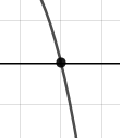
\includegraphics[width = 0.3\textwidth]{../Figures/polyZeroBehaviorCopyAA.png}\item 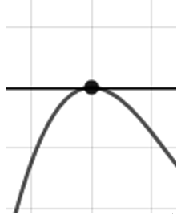
\includegraphics[width = 0.3\textwidth]{../Figures/polyZeroBehaviorCopyBA.png}\item 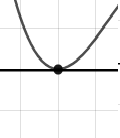
\includegraphics[width = 0.3\textwidth]{../Figures/polyZeroBehaviorCopyCA.png}\item 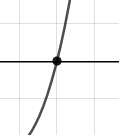
\includegraphics[width = 0.3\textwidth]{../Figures/polyZeroBehaviorCopyDA.png}\end{multicols}\item None of the above.
\end{enumerate} }
\litem{
Construct the lowest-degree polynomial given the zeros below. Then, choose the intervals that contain the coefficients of the polynomial in the form $ax^3+bx^2+cx+d$.\[ \frac{5}{3}, 7, \text{ and } \frac{-7}{5} \]\begin{enumerate}[label=\Alph*.]
\item \( a \in [13, 24], b \in [143, 153], c \in [348, 358], \text{ and } d \in [239, 253] \)
\item \( a \in [13, 24], b \in [-110, -101], c \in [-10, -4], \text{ and } d \in [239, 253] \)
\item \( a \in [13, 24], b \in [-110, -101], c \in [-10, -4], \text{ and } d \in [-247, -238] \)
\item \( a \in [13, 24], b \in [106, 114], c \in [-10, -4], \text{ and } d \in [-247, -238] \)
\item \( a \in [13, 24], b \in [-60, -56], c \in [-287, -277], \text{ and } d \in [-247, -238] \)

\end{enumerate} }
\litem{
Which of the following equations \textit{could} be of the graph presented below?
\begin{center}
    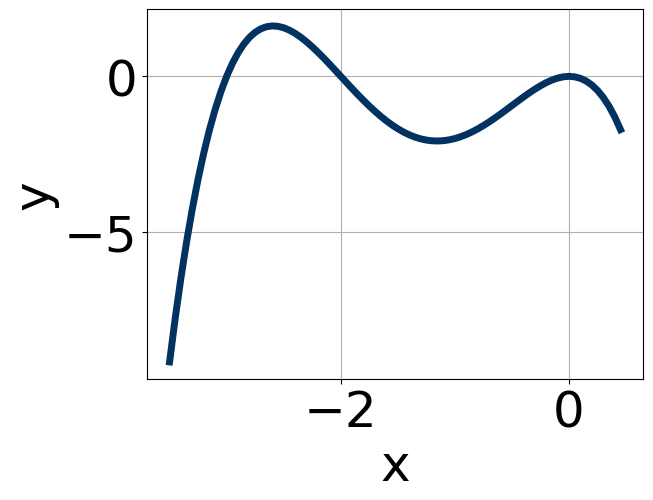
\includegraphics[width=0.5\textwidth]{../Figures/polyGraphToFunctionCopyA.png}
\end{center}
\begin{enumerate}[label=\Alph*.]
\item \( 9x^{4} (x + 3)^{7} (x + 2)^{11} \)
\item \( -20x^{10} (x + 3)^{10} (x + 2)^{11} \)
\item \( 14x^{4} (x + 3)^{9} (x + 2)^{8} \)
\item \( -13x^{9} (x + 3)^{6} (x + 2)^{9} \)
\item \( -18x^{6} (x + 3)^{11} (x + 2)^{9} \)

\end{enumerate} }
\litem{
Construct the lowest-degree polynomial given the zeros below. Then, choose the intervals that contain the coefficients of the polynomial in the form $x^3+bx^2+cx+d$.\[ 5 - 3 i \text{ and } 2 \]\begin{enumerate}[label=\Alph*.]
\item \( b \in [-9, 6], c \in [0, 6], \text{ and } d \in [-9, 1] \)
\item \( b \in [10, 13], c \in [52, 62], \text{ and } d \in [68, 76] \)
\item \( b \in [-14, -11], c \in [52, 62], \text{ and } d \in [-76, -62] \)
\item \( b \in [-9, 6], c \in [-13, -1], \text{ and } d \in [4, 16] \)
\item \( \text{None of the above.} \)

\end{enumerate} }
\litem{
Describe the end behavior of the polynomial below.\[ f(x) = 8(x + 3)^{3}(x - 3)^{8}(x - 2)^{3}(x + 2)^{4} \]\begin{enumerate}[label=\Alph*.]
\begin{multicols}{2}\item 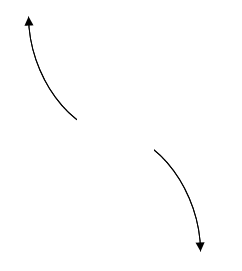
\includegraphics[width = 0.3\textwidth]{../Figures/polyEndBehaviorAB.png}\item 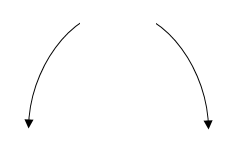
\includegraphics[width = 0.3\textwidth]{../Figures/polyEndBehaviorBB.png}\item 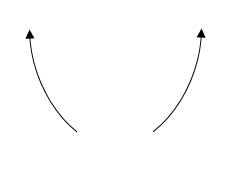
\includegraphics[width = 0.3\textwidth]{../Figures/polyEndBehaviorCB.png}\item 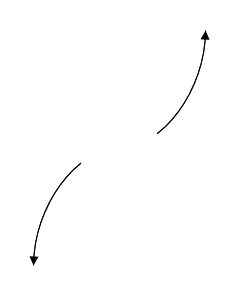
\includegraphics[width = 0.3\textwidth]{../Figures/polyEndBehaviorDB.png}\end{multicols}\item None of the above.
\end{enumerate} }
\litem{
Describe the end behavior of the polynomial below.\[ f(x) = 7(x - 4)^{4}(x + 4)^{5}(x + 3)^{3}(x - 3)^{5} \]\begin{enumerate}[label=\Alph*.]
\begin{multicols}{2}\item 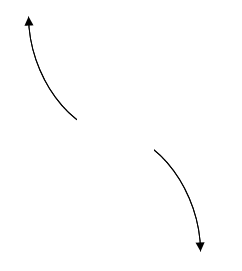
\includegraphics[width = 0.3\textwidth]{../Figures/polyEndBehaviorCopyAB.png}\item 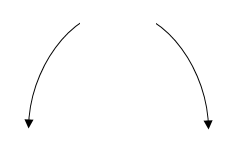
\includegraphics[width = 0.3\textwidth]{../Figures/polyEndBehaviorCopyBB.png}\item 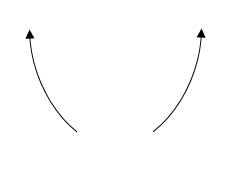
\includegraphics[width = 0.3\textwidth]{../Figures/polyEndBehaviorCopyCB.png}\item 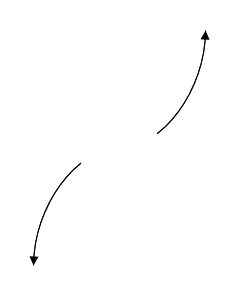
\includegraphics[width = 0.3\textwidth]{../Figures/polyEndBehaviorCopyDB.png}\end{multicols}\item None of the above.
\end{enumerate} }
\litem{
Construct the lowest-degree polynomial given the zeros below. Then, choose the intervals that contain the coefficients of the polynomial in the form $ax^3+bx^2+cx+d$.\[ 7, \frac{-1}{5}, \text{ and } \frac{2}{3} \]\begin{enumerate}[label=\Alph*.]
\item \( a \in [15, 17], b \in [110.6, 112.3], c \in [44, 57], \text{ and } d \in [-17, -12] \)
\item \( a \in [15, 17], b \in [91.8, 95.9], c \in [-92, -82], \text{ and } d \in [14, 19] \)
\item \( a \in [15, 17], b \in [-112.5, -108.4], c \in [44, 57], \text{ and } d \in [14, 19] \)
\item \( a \in [15, 17], b \in [96, 100.8], c \in [-52, -44], \text{ and } d \in [-17, -12] \)
\item \( a \in [15, 17], b \in [-112.5, -108.4], c \in [44, 57], \text{ and } d \in [-17, -12] \)

\end{enumerate} }
\litem{
Describe the zero behavior of the zero $x = 2$ of the polynomial below.\[ f(x) = -3(x + 2)^{4}(x - 2)^{5}(x - 7)^{5}(x + 7)^{7} \]\begin{enumerate}[label=\Alph*.]
\begin{multicols}{2}\item 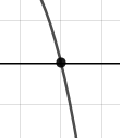
\includegraphics[width = 0.3\textwidth]{../Figures/polyZeroBehaviorAB.png}\item 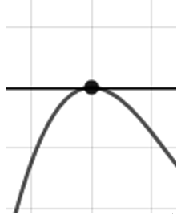
\includegraphics[width = 0.3\textwidth]{../Figures/polyZeroBehaviorBB.png}\item 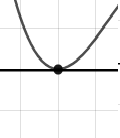
\includegraphics[width = 0.3\textwidth]{../Figures/polyZeroBehaviorCB.png}\item 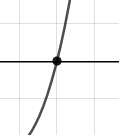
\includegraphics[width = 0.3\textwidth]{../Figures/polyZeroBehaviorDB.png}\end{multicols}\item None of the above.
\end{enumerate} }
\litem{
Which of the following equations \textit{could} be of the graph presented below?
\begin{center}
    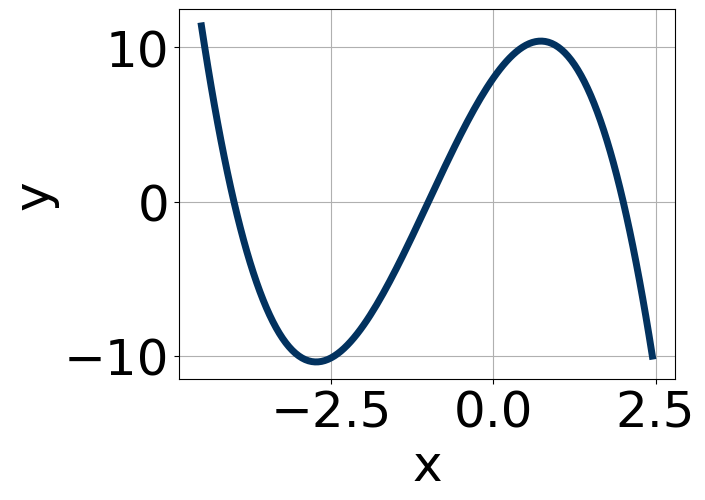
\includegraphics[width=0.5\textwidth]{../Figures/polyGraphToFunctionB.png}
\end{center}
\begin{enumerate}[label=\Alph*.]
\item \( -8(x - 2)^{10} (x + 4)^{6} (x + 1)^{5} \)
\item \( 12(x - 2)^{8} (x + 4)^{7} (x + 1)^{7} \)
\item \( -4(x - 2)^{10} (x + 4)^{11} (x + 1)^{11} \)
\item \( 11(x - 2)^{7} (x + 4)^{9} (x + 1)^{9} \)
\item \( -10(x - 2)^{5} (x + 4)^{7} (x + 1)^{11} \)

\end{enumerate} }
\litem{
Construct the lowest-degree polynomial given the zeros below. Then, choose the intervals that contain the coefficients of the polynomial in the form $x^3+bx^2+cx+d$.\[ 4 + 5 i \text{ and } 1 \]\begin{enumerate}[label=\Alph*.]
\item \( b \in [-11, -5], c \in [48.79, 49.11], \text{ and } d \in [-41.09, -39.64] \)
\item \( b \in [1, 6], c \in [-5.16, -3.28], \text{ and } d \in [2.13, 4.62] \)
\item \( b \in [1, 6], c \in [-6.36, -5.54], \text{ and } d \in [4.44, 5.18] \)
\item \( b \in [3, 14], c \in [48.79, 49.11], \text{ and } d \in [39.48, 43] \)
\item \( \text{None of the above.} \)

\end{enumerate} }
\litem{
Describe the zero behavior of the zero $x = -7$ of the polynomial below.\[ f(x) = -9(x - 4)^{5}(x + 4)^{2}(x + 7)^{11}(x - 7)^{8} \]\begin{enumerate}[label=\Alph*.]
\begin{multicols}{2}\item 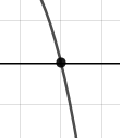
\includegraphics[width = 0.3\textwidth]{../Figures/polyZeroBehaviorCopyAB.png}\item 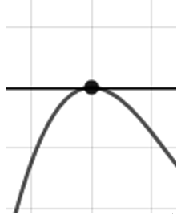
\includegraphics[width = 0.3\textwidth]{../Figures/polyZeroBehaviorCopyBB.png}\item 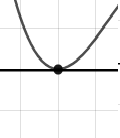
\includegraphics[width = 0.3\textwidth]{../Figures/polyZeroBehaviorCopyCB.png}\item 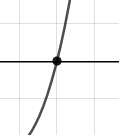
\includegraphics[width = 0.3\textwidth]{../Figures/polyZeroBehaviorCopyDB.png}\end{multicols}\item None of the above.
\end{enumerate} }
\litem{
Construct the lowest-degree polynomial given the zeros below. Then, choose the intervals that contain the coefficients of the polynomial in the form $ax^3+bx^2+cx+d$.\[ -1, \frac{-4}{5}, \text{ and } \frac{3}{5} \]\begin{enumerate}[label=\Alph*.]
\item \( a \in [19, 32], b \in [28, 33], c \in [-10, -3], \text{ and } d \in [12, 19] \)
\item \( a \in [19, 32], b \in [-26, -18], c \in [-20, -16], \text{ and } d \in [12, 19] \)
\item \( a \in [19, 32], b \in [-64, -56], c \in [45, 49], \text{ and } d \in [-12, -9] \)
\item \( a \in [19, 32], b \in [28, 33], c \in [-10, -3], \text{ and } d \in [-12, -9] \)
\item \( a \in [19, 32], b \in [-32, -26], c \in [-10, -3], \text{ and } d \in [12, 19] \)

\end{enumerate} }
\litem{
Which of the following equations \textit{could} be of the graph presented below?
\begin{center}
    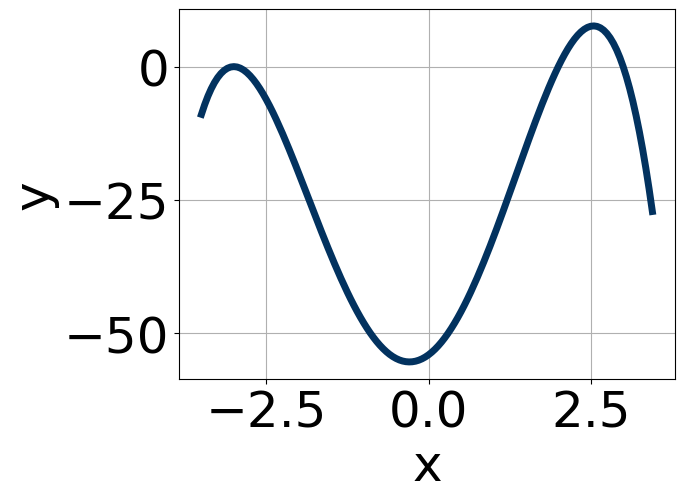
\includegraphics[width=0.5\textwidth]{../Figures/polyGraphToFunctionCopyB.png}
\end{center}
\begin{enumerate}[label=\Alph*.]
\item \( 12(x + 3)^{8} (x - 2)^{11} (x - 3)^{9} \)
\item \( -19(x + 3)^{6} (x - 2)^{10} (x - 3)^{11} \)
\item \( -20(x + 3)^{9} (x - 2)^{6} (x - 3)^{9} \)
\item \( 6(x + 3)^{4} (x - 2)^{11} (x - 3)^{4} \)
\item \( -5(x + 3)^{6} (x - 2)^{5} (x - 3)^{9} \)

\end{enumerate} }
\litem{
Construct the lowest-degree polynomial given the zeros below. Then, choose the intervals that contain the coefficients of the polynomial in the form $x^3+bx^2+cx+d$.\[ 5 + 2 i \text{ and } 1 \]\begin{enumerate}[label=\Alph*.]
\item \( b \in [-18, -7], c \in [35.4, 40.7], \text{ and } d \in [-30.8, -28.8] \)
\item \( b \in [-6, 7], c \in [-10.4, -5.5], \text{ and } d \in [2.6, 6.3] \)
\item \( b \in [-6, 7], c \in [-4.6, -2.6], \text{ and } d \in [-4.2, 2.7] \)
\item \( b \in [10, 12], c \in [35.4, 40.7], \text{ and } d \in [24.9, 29.1] \)
\item \( \text{None of the above.} \)

\end{enumerate} }
\litem{
Describe the end behavior of the polynomial below.\[ f(x) = 7(x - 4)^{3}(x + 4)^{4}(x - 8)^{2}(x + 8)^{2} \]\begin{enumerate}[label=\Alph*.]
\begin{multicols}{2}\item 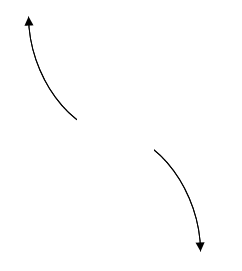
\includegraphics[width = 0.3\textwidth]{../Figures/polyEndBehaviorAC.png}\item 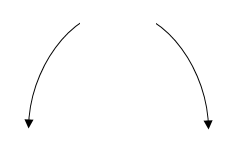
\includegraphics[width = 0.3\textwidth]{../Figures/polyEndBehaviorBC.png}\item 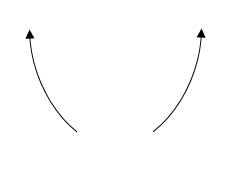
\includegraphics[width = 0.3\textwidth]{../Figures/polyEndBehaviorCC.png}\item 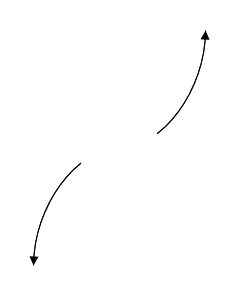
\includegraphics[width = 0.3\textwidth]{../Figures/polyEndBehaviorDC.png}\end{multicols}\item None of the above.
\end{enumerate} }
\litem{
Describe the end behavior of the polynomial below.\[ f(x) = 4(x + 3)^{2}(x - 3)^{7}(x + 8)^{5}(x - 8)^{6} \]\begin{enumerate}[label=\Alph*.]
\begin{multicols}{2}\item 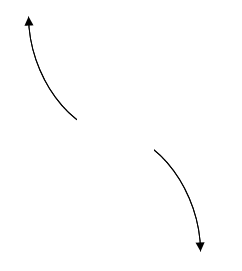
\includegraphics[width = 0.3\textwidth]{../Figures/polyEndBehaviorCopyAC.png}\item 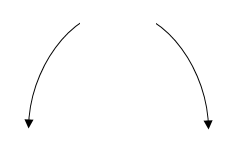
\includegraphics[width = 0.3\textwidth]{../Figures/polyEndBehaviorCopyBC.png}\item 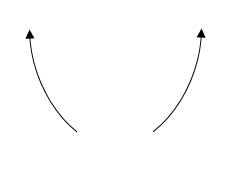
\includegraphics[width = 0.3\textwidth]{../Figures/polyEndBehaviorCopyCC.png}\item 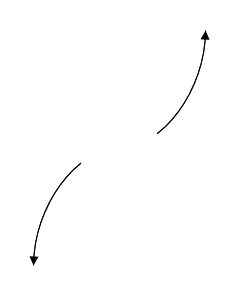
\includegraphics[width = 0.3\textwidth]{../Figures/polyEndBehaviorCopyDC.png}\end{multicols}\item None of the above.
\end{enumerate} }
\litem{
Construct the lowest-degree polynomial given the zeros below. Then, choose the intervals that contain the coefficients of the polynomial in the form $ax^3+bx^2+cx+d$.\[ \frac{-3}{4}, -7, \text{ and } \frac{-1}{3} \]\begin{enumerate}[label=\Alph*.]
\item \( a \in [12, 14], b \in [94, 98], c \in [90, 105], \text{ and } d \in [20, 26] \)
\item \( a \in [12, 14], b \in [-99, -94], c \in [90, 105], \text{ and } d \in [-26, -20] \)
\item \( a \in [12, 14], b \in [-93, -88], c \in [31, 33], \text{ and } d \in [20, 26] \)
\item \( a \in [12, 14], b \in [78, 86], c \in [-43, -37], \text{ and } d \in [-26, -20] \)
\item \( a \in [12, 14], b \in [94, 98], c \in [90, 105], \text{ and } d \in [-26, -20] \)

\end{enumerate} }
\litem{
Describe the zero behavior of the zero $x = -9$ of the polynomial below.\[ f(x) = 2(x - 4)^{10}(x + 4)^{6}(x + 9)^{10}(x - 9)^{7} \]\begin{enumerate}[label=\Alph*.]
\begin{multicols}{2}\item 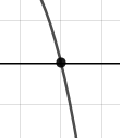
\includegraphics[width = 0.3\textwidth]{../Figures/polyZeroBehaviorAC.png}\item 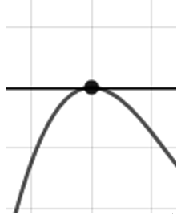
\includegraphics[width = 0.3\textwidth]{../Figures/polyZeroBehaviorBC.png}\item 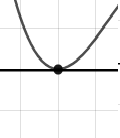
\includegraphics[width = 0.3\textwidth]{../Figures/polyZeroBehaviorCC.png}\item 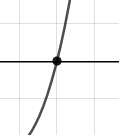
\includegraphics[width = 0.3\textwidth]{../Figures/polyZeroBehaviorDC.png}\end{multicols}\item None of the above.
\end{enumerate} }
\litem{
Which of the following equations \textit{could} be of the graph presented below?
\begin{center}
    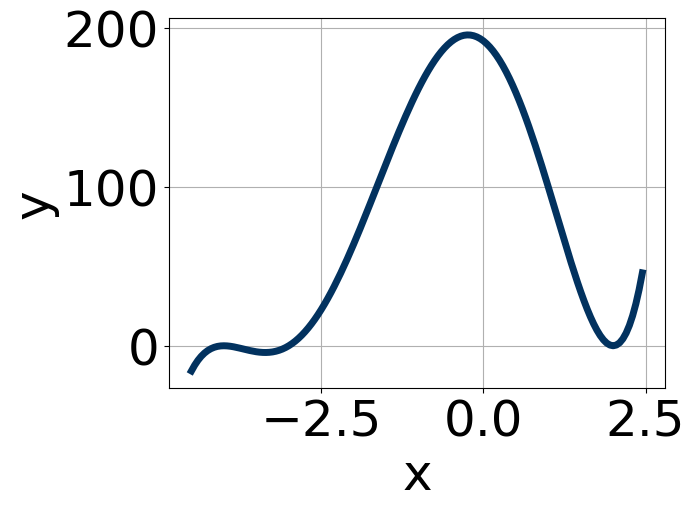
\includegraphics[width=0.5\textwidth]{../Figures/polyGraphToFunctionC.png}
\end{center}
\begin{enumerate}[label=\Alph*.]
\item \( 15(x + 4)^{6} (x - 2)^{7} (x + 3)^{5} \)
\item \( -6(x + 4)^{10} (x - 2)^{6} (x + 3)^{8} \)
\item \( 17(x + 4)^{10} (x - 2)^{7} (x + 3)^{10} \)
\item \( -19(x + 4)^{8} (x - 2)^{8} (x + 3)^{7} \)
\item \( 6(x + 4)^{4} (x - 2)^{8} (x + 3)^{7} \)

\end{enumerate} }
\litem{
Construct the lowest-degree polynomial given the zeros below. Then, choose the intervals that contain the coefficients of the polynomial in the form $x^3+bx^2+cx+d$.\[ 2 + 3 i \text{ and } 1 \]\begin{enumerate}[label=\Alph*.]
\item \( b \in [-1.8, 1.9], c \in [-4.15, -3.21], \text{ and } d \in [2.99, 3.53] \)
\item \( b \in [-9.1, -3.5], c \in [16.78, 18.65], \text{ and } d \in [-14.03, -11.89] \)
\item \( b \in [4.7, 5.3], c \in [16.78, 18.65], \text{ and } d \in [11.64, 13.41] \)
\item \( b \in [-1.8, 1.9], c \in [-3.38, -1.37], \text{ and } d \in [1.75, 2.85] \)
\item \( \text{None of the above.} \)

\end{enumerate} }
\litem{
Describe the zero behavior of the zero $x = -4$ of the polynomial below.\[ f(x) = 6(x - 4)^{7}(x + 4)^{12}(x + 3)^{4}(x - 3)^{6} \]\begin{enumerate}[label=\Alph*.]
\begin{multicols}{2}\item 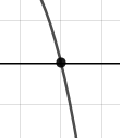
\includegraphics[width = 0.3\textwidth]{../Figures/polyZeroBehaviorCopyAC.png}\item \includegraphics[width = 0.3\textwidth]{../Figures/polyZeroBehaviorCopyBC.png}\item \includegraphics[width = 0.3\textwidth]{../Figures/polyZeroBehaviorCopyCC.png}\item \includegraphics[width = 0.3\textwidth]{../Figures/polyZeroBehaviorCopyDC.png}\end{multicols}\item None of the above.
\end{enumerate} }
\litem{
Construct the lowest-degree polynomial given the zeros below. Then, choose the intervals that contain the coefficients of the polynomial in the form $ax^3+bx^2+cx+d$.\[ \frac{1}{2}, \frac{5}{4}, \text{ and } \frac{-1}{5} \]\begin{enumerate}[label=\Alph*.]
\item \( a \in [37, 43], b \in [-63, -59], c \in [10, 12], \text{ and } d \in [4, 9] \)
\item \( a \in [37, 43], b \in [-24, -15], c \in [-38, -26], \text{ and } d \in [-12, -4] \)
\item \( a \in [37, 43], b \in [-63, -59], c \in [10, 12], \text{ and } d \in [-12, -4] \)
\item \( a \in [37, 43], b \in [74, 85], c \in [38, 41], \text{ and } d \in [4, 9] \)
\item \( a \in [37, 43], b \in [55, 66], c \in [10, 12], \text{ and } d \in [-12, -4] \)

\end{enumerate} }
\litem{
Which of the following equations \textit{could} be of the graph presented below?
\begin{center}
    \includegraphics[width=0.5\textwidth]{../Figures/polyGraphToFunctionCopyC.png}
\end{center}
\begin{enumerate}[label=\Alph*.]
\item \( -2x^{8} (x - 1)^{5} (x + 2)^{7} \)
\item \( 13x^{9} (x - 1)^{4} (x + 2)^{9} \)
\item \( -14x^{8} (x - 1)^{7} (x + 2)^{10} \)
\item \( 4x^{4} (x - 1)^{11} (x + 2)^{11} \)
\item \( 7x^{8} (x - 1)^{6} (x + 2)^{7} \)

\end{enumerate} }
\end{enumerate}

\end{document}